\subsection*{Función óxido}
Los óxidos son compuestos binarios formados por combinación química del oxi9dgeno con otro elemento u compuesto. 
\subsubsection*{Óxidos básicos}
Son aquellos formados por la combinación química del oxigeno con metales. Estos compuestos son generalmente sólidos a temperatura ambiente y poseen enlace iónico.
\begin{Theorem*} {Óxidos básicos}
	\begin{figure}[H]
		\centering
		\begin{tikzpicture}
			\node at (0,3) {$\text{Metal} + \mathrm{O}^{-2} \rightarrow \text{Óxido Básico}$};
			\draw[<-] (-2,2.7) -- (-2,2.5);
			\draw (-2,2.5) -- (-4,2.5);
			\draw (-4,2.5) -- (-4, 1.8);
			\draw[->] (-4,1.8) -- (-3.6, 1.8);
			\draw (-3.5,2.2) -- (-3.5, 1.3);
			\node[anchor=mid west] at (-3.5,2) {- Cualquier metal};
			\node[anchor=mid west] at (-3.5,1.5) {- Anfóteros con +2 +3};
		\end{tikzpicture}
	\end{figure}
	$$\ch{M^{+} + O^{-2} ->}\mathrm{M}_2\mathrm{O}_x$$
\end{Theorem*}
\noindent Ejemplos
\begin{align*}
	&\ch{"\ox{+1,Na}" + "\ox{-2,O}" -> Na2O}\left\{\begin{array}{l}
		\text{T: óxido de sodio}\\
		\text{S: óxido de sodio (I)}\\
		\text{I: monóxido de disodio}
	\end{array}\right. \\
	&\ch{"\ox{+2,Fe}" + "\ox{-2,O}" -> Fe2O2 -> FeO}\left\{\begin{array}{l}
		\text{T: óxido ferroso}\\
		\text{S: óxido de hierro (II)}\\
		\text{I: monóxido de hierro}
	\end{array}\right.\\
	&\ch{"\ox{+3,Fe}" + "\ox{-2,O}" -> Fe2O3}\left\{\begin{array}{l}
		\text{T: óxido ferroso}\\
		\text{S: óxido de hierro (III)}\\
		\text{I: trióxido de dihierro}
	\end{array}\right.\\
	&\ch{"\ox{+2,Cr}" + "\ox{-2,O}" -> CrO}\left\{\begin{array}{l}
		\text{T: óxido cromoso}\\
		\text{S: óxido de cromo (II)}\\
		\text{I: monoóxido de cromo}
	\end{array}\right.\\
	&\ch{"\ox{+3,Cr}" + "\ox{-2,O}" -> Cr2O3}\left\{\begin{array}{l}
		\text{T: óxido crómico}\\
		\text{S: óxido de cromo (III)}\\
		\text{I: trióxido de dicromo}
	\end{array}\right.\\
	&\ch{"\ox{+4,Pb}" + "\ox{-2,O}" -> PbO2}\left\{\begin{array}{l}
		\text{T: óxido plumbico}\\
		\text{S: óxido de plomo (IV)}\\
		\text{I: dióxido de plomo}
	\end{array}\right.\\
	&\ch{"\ox{+1,Au}" + "\ox{-2,O}" -> Au2O}\left\{\begin{array}{l}
		\text{T: óxido auroso}\\
		\text{S: óxido de oro (I)}\\
		\text{I: monóxido de dioro}
	\end{array}\right.\\
	&\ch{"\ox{+2,Cu}" + "\ox{-2,O}" -> CuO}\left\{\begin{array}{l}
		\text{T: óxido cúprico}\\
		\text{S: óxido de cobre (II)}\\
		\text{I: monóxido de cobre}
	\end{array}\right.\\
	&\ch{"\ox{+1,Hg}" + "\ox{-2,O}" -> Hg2O}\left\{\begin{array}{l}
		\text{T: óxido mercurioso}\\
		\text{S: óxido de mercurio (I)}\\
		\text{I: monóxido de dimercurio}
	\end{array}\right.\\
	&\ch{"\ox{+2,Hg}" + "\ox{-2,O}" -> HgO}\left\{\begin{array}{l}
		\text{T: óxido mercúrico}\\
		\text{S: óxido de mercurio (II)}\\
		\text{I: monóxido de mercurio}
	\end{array}\right.\\
\end{align*}
\subsubsection*{Óxidos ácidos o anhídridos}
Son óxidos formados por la combinación del oxigeno con elementos no metálicos, aunque también se encuentran en esta categoría algunos óxidos de metales que son anfóteros como el Vanadio, Cromo y manganeso. En la nomenclatura tradicional se denomina anhídrido que quiere decir sin $\ch{H2O}$ que es el nombre genérico seguido del nombre del elemento.
\begin{Theorem*} {Anhídridos}
	\begin{figure}[H]
		\centering
		\begin{tikzpicture}
			\node at (0,3) {$\text{No Metal} + \mathrm{O}^{-2} \rightarrow \text{Anhídrido}$};
			\draw[<-] (-2,2.7) -- (-2,2.5);
			\draw (-2,2.5) -- (-4,2.5);
			\draw (-4,2.5) -- (-4, 1.8);
			\draw[->] (-4,1.8) -- (-3.6, 1.8);
			\draw (-3.5,2.2) -- (-3.5, 1.3);
			\node[anchor=mid west] at (-3.5,2) {- Cualquier no metal};
			\node[anchor=mid west] at (-3.5,1.5) {- Anfóteros con +5 +6 +7};
		\end{tikzpicture}
	\end{figure}
	$$\ch{NM^{+} + O^{-2} ->}\mathrm{NM}_2\mathrm{O}_x$$
\end{Theorem*}
\noindent Ejemplos:
\begin{align*}
	&\ch{"\ox{+1,Cl}" + "\ox{-2,O}" -> Cl2O}\left\{\begin{array}{l}
		\text{T: anhídrido hipocloroso}\\
		\text{S: óxido de cloro (I)}\\
		\text{I: monóxido de dicloro}
	\end{array}\right.\\
	&\ch{"\ox{+3,Br}" + "\ox{-2,O}" -> Br2O3}\left\{\begin{array}{l}
		\text{T: anhídrido bromoso}\\
		\text{S: óxido de bromo (III)}\\
		\text{I: trióxido de dibromo}
	\end{array}\right.\\
	&\ch{"\ox{+5,I}" + "\ox{-2,O}" -> I2O5}\left\{\begin{array}{l}
		\text{T: anhídrido yódico}\\
		\text{S: óxido de yodo (V)}\\
		\text{I: pentaóxido de diyodo}
	\end{array}\right.\\
	&\ch{"\ox{+7,Cl}" + "\ox{-2,O}" -> Cl2O7}\left\{\begin{array}{l}
		\text{T: anhídrido perclórico}\\
		\text{S: óxido de cloro (VII)}\\
		\text{I: heptaóxido de dicloro}
	\end{array}\right.\\
	&\ch{"\ox{+3,B}" + "\ox{-2,O}" -> B2O3}\left\{\begin{array}{l}
		\text{T: anhídrido bórico}\\
		\text{S: óxido de boro (III)}\\
		\text{I: trióxido de diboro}
	\end{array}\right.\\
	&\ch{"\ox{+2,C}" + "\ox{-2,O}" -> CO}\left\{\begin{array}{l}
		\text{T: anhídrido carbonoso}\\
		\text{S: óxido de carbono (II)}\\
		\text{I: monóxido de carbono}
	\end{array}\right.\\
	&\ch{"\ox{+6,S}" + "\ox{-2,O}" -> SO3}\left\{\begin{array}{l}
		\text{T: anhídrido sulfúrico}\\
		\text{S: óxido de azufre (VI)}\\
		\text{I: trióxido de azufre}
	\end{array}\right.\\
	&\ch{"\ox{+3,N}" + "\ox{-2,O}" -> N2O3}\left\{\begin{array}{l}
		\text{T: anhídrido nitroso}\\
		\text{S: óxido de nitrógeno (III)}\\
		\text{I: trióxido de dinitrógeno}
	\end{array}\right.\\
	&\ch{"\ox{+5,N}" + "\ox{-2,O}" -> N2O5}\left\{\begin{array}{l}
		\text{T: anhídrido nítrico}\\
		\text{S: óxido de nitrógeno (V)}\\
		\text{I: pentaóxido de dinitrógeno}
	\end{array}\right.\\
	\intertext{Casos especial del nitrogeno: }
	&\ch{"\ox{+1,N}" + "\ox{-2,O}" -> N2O}\left\{\begin{array}{l}
		\text{T: anhídrido hiponitroso}\\
		\text{T: óxido nitroso}\\
		\text{S: óxido de nitrógeno (I)}\\
		\text{I: monóxido de dinitrógeno}
	\end{array}\right.\\
	&\ch{"\ox{+2,N}" + "\ox{-2,O}" -> NO}\left\{\begin{array}{l}
		\text{T: oxido nitroso}\\
		\text{S: óxido de nitrógeno (II)}\\
		\text{I: monóxido de nitrógeno}
	\end{array}\right.\\
	\intertext{casos especiales de la valencia +4}
	&\ch{"\ox{+4,N}" + "\ox{-2,O}" -> NO2}\left\{\begin{array}{l}
		\text{T: óxido nítrico}\\
		\text{S: óxido de nitrógeno (IV)}\\
		\text{I: dióxido de nitrógeno}
	\end{array}\right.\\
	&\ch{"\ox{+4,Mn}" + "\ox{-2,O}" -> MnO2}\left\{\begin{array}{l}
		\text{T: anhídrido manganoso}\\
		\text{S: óxido de de manganeso (IV)}\\
		\text{I: dióxido de manganeso}
	\end{array}\right.\\
	&\ch{"\ox{+4,Mo}" + "\ox{-2,O}" -> MoO2}\left\{\begin{array}{l}
		\text{S: óxido de molibdeno (IV)}\\
		\text{I: dióxido de molibdeno}
	\end{array}\right.\\
	&\ch{"\ox{+4,W}" + "\ox{-2,O}" -> WO2}\left\{\begin{array}{l}
		\text{S: óxido de wolframio (IV)}\\
		\text{I: dióxido de wolframio}
	\end{array}\right.\\
	&\ch{"\ox{+4,Ti}" + "\ox{-2,O}" -> TiO2}\left\{\begin{array}{l}
		\text{T: óxido titánico}\\
		\text{S: óxido de titanio (IV)}\\
		\text{I: dióxido de titanio}
	\end{array}\right.\\
	&\ch{"\ox{+1,U}" + "\ox{-2,O}" -> UO2}\left\{\begin{array}{l}
		\text{T: óxido uranioso}\\
		\text{S: óxido de uranio (IV)}\\
		\text{I: dióxido de uranio}
	\end{array}\right.\\
\end{align*}
\subsubsection*{Superóxidos o hiperóxidos}
Un superóxido o hiperóxido es un compuesto binario que contiene el anión superóxido O2-. Se considera que el oxígeno ,que siempre tiene valencia 2, tiene valencia 1/2.
\begin{Theorem*} {Superóxidos}
	\begin{figure}[H]
		\centering
		\begin{tikzpicture}
			\node at (0,3) {$\text{Metal} + \mathrm{O}^{-}_{2} \rightarrow \text{Superóxido}$};
			\draw[<-] (-2,2.7) -- (-2,2.5);
			\draw (-2,2.5) -- (-4,2.5);
			\draw (-4,2.5) -- (-4, 1.8);
			\draw[->] (-4,1.8) -- (-3.6, 1.8);
			
			\draw (-3.5,2.2) -- (-3.5, 0.8);
			
			\node[anchor=mid west] at (-3.5,2) {- monovalentes};
			\node[anchor=mid west] at (-3.5,1.5) {- bivalentes};
			\node[anchor=mid west] at (-3.5,1) {- trivalentes};
		\end{tikzpicture}
	\end{figure}
	$$\mathrm{M}^{+} + \mathrm{O}^{-1}_2 \rightarrow\mathrm{M}\mathrm{O}_{2x} $$
	o también:
	$$\mathrm{M}^{+} + \mathrm{O}^{-\frac{1}{2}} \rightarrow2\mathrm{M}_{\frac{1}{2}}\mathrm{O}_x\rightarrow\mathrm{M}\mathrm{O}_{2x} $$
\end{Theorem*}
\noindent ejemplos:
\begin{align*}
	&\ch{"\ox{+1,Li}" + "\ox{-1,O2}" -> LiO2} \ \text{\{ T: superóxido de litio}\\
	&\ch{"\ox{+2,Ca}" + "\ox{-1,O2}" -> CaO4} \ \text{\{ T: superóxido de calcio}\\
	&\ch{"\ox{+3,Al}" + "\ox{-1,O2}" -> AlO6} \ \text{\{ T: superóxido de aluminio}
\end{align*}
\subsubsection*{Peróxidos}
Son compuestos binarios iónicos, generalmente, que forma el oxigeno con algunos metales, principales de los grupos 1A y 11A. Se caracterizan por la presencia del ion peróxido ($\ch{"\ox{-2, O2}"}$) donde se puede evaluar que cada una átomo de oxigeno actúa con E.O. igual a -1. En el caso de que un metal posee varias valencias, el peróxido solo es estable con la mayor valencia del metal, porque el metal sufre una oxidacion profunda al formar el peróxido.
\begin{Theorem*} {Peróxidos}
	\begin{figure}[H]
		\centering
		\begin{tikzpicture}
			\node at (0,3) {$\text{óxido básico} + \mathrm{O} \rightarrow \text{peróxido}$};
			\draw[<-] (-2,2.7) -- (-2,2.5);
			\draw (-2,2.5) -- (-4,2.5);
			\draw (-4,2.5) -- (-4, 1.8);
			\draw[->] (-4,1.8) -- (-3.6, 1.8);
			
			\draw (-3.5,2.2) -- (-3.5, 1.3);
			
			\node[anchor=mid west] at (-3.5,2) {- monovalentes};
			\node[anchor=mid west] at (-3.5,1.5) {- bivalentes};
		\end{tikzpicture}
	\end{figure}
	$$\mathrm{O.B.} + \mathrm{O} \rightarrow\mathrm{M}_2\mathrm{O}_2 \quad (\text{Si es monovalente}) $$
	$$\mathrm{O.B.} + \mathrm{O} \rightarrow\mathrm{M}\mathrm{O}_2 \quad (\text{Si es bivalente}) $$
\end{Theorem*}
\noindent ejemplos:
\begin{align*}
	&\ch{Li2O + O -> Li2O2} \ \text{\{ T: peróxido de litio}\\
	&\ch{Na2O + O -> CaO4} \ \text{\{ T: peróxido de sodio}\\
	&\ch{CaO + O -> CaO2} \ \text{\{ T: peróxido de calcio}\\
	&\ch{SrO + O -> SrO2} \ \text{\{ T: peróxido de estroncio}
	\intertext{casos especiales:}
	&\ch{H2O + O -> H2O2}\left\{\begin{array}{l}
		\text{T: peróxido de hidrógeno}\\
		\text{C: agua oxigenada}
	\end{array}\right.\\
	&\ch{"\ox{+4,N}" + O -> N2O4} \ \text{\{ T: peróxido de nitrógeno} \\
	&\ch{Hg2O + O -> Hg2O2} \ \text{\{ T: peróxido mercurioso}
\end{align*}
\subsubsection*{Óxidos salinos o dobles}
Son compuestos que forma el oxigeno con algunos metales como Fe, Pb, Co, Ni, etc. Debido a la combinación de metales +2+3 o +2+4 generalmente la formula es $\ch{M3O4}$, sin embargo existe casos especiales como se vera después.
\begin{Theorem*} {Óxidos dobles}
	\begin{figure}[H]
		\centering
		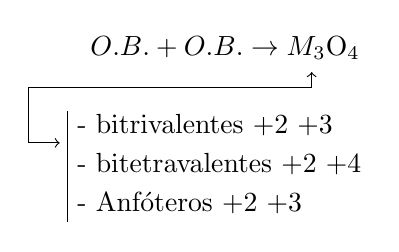
\begin{tikzpicture}
			\node at (-1.5,3) {$\text{O.B.}+\text{O.B.}\rightarrow\text{M}_3 \mathrm{O}_4$};
			\draw[<-] (-0.4,2.7) -- (-0.4,2.5);
			\draw (-0.4,2.5) -- (-4,2.5);
			\draw (-4,2.5) -- (-4, 1.8);
			\draw[->] (-4,1.8) -- (-3.6, 1.8);
			
			\draw (-3.5,2.2) -- (-3.5, 0.8);
			
			\node[anchor=mid west] at (-3.5,2) {- bitrivalentes +2 +3};
			\node[anchor=mid west] at (-3.5,1.5) {- bitetravalentes +2 +4};
			\node[anchor=mid west] at (-3.5,1) {- Anfóteros +2 +3};
		\end{tikzpicture}
	\end{figure}
	\begin{flalign*}
		&\begin{array} {ll}
			\ \ M \ O\\
			+MO_2\\\hline
			\ M_3O_4
		\end{array} \quad \begin{array} {ll}
		\ 2M \ O\\
		+M_2O_3\\\hline
		\ M_3O_4
		\end{array}
	\end{flalign*}
\end{Theorem*}
Ejemplos
\begin{align*}
	&\begin{array} {rl}
		\ch{FeO} & \text{óxdio ferroso} \\
		\ch{Fe2O3} & \text{óxdio férrico} \\ \hline
		\ch{Fe3O4} & \begin{array} {l}
			\text{T: óxido ferroso-férrico} \\
			\text{T: óxido salino de hierro} \\
			\text{T: óxido doble de hierro} \\
			\text{T: óxidos mixto de hierro} \\
			\text{S: óxido de hierro (II y III)} \\
			\text{I: tetraóxido de trihierro}
		\end{array}
	\end{array} \\
	&\begin{array} {rl}
		\ch{2 SnO} & \text{óxdio estanoso} \\
		\ch{SnO2} & \text{óxdio estánico} \\ \hline
		\ch{Sn3O4} & \begin{array} {l}
			\text{T: óxido estanoso-estánico} \\
			\text{T: óxido salino de estaño} \\
			\text{T: óxido doble de estaño} \\
			\text{T: óxidos mixto de estaño} \\
			\text{S: óxido de estaño (II y III)} \\
			\text{I: tetraóxido de triestaño}
		\end{array}
	\end{array}
	\intertext{casos especiales del 38}
	&\ch{U3O8} \ \text{\{ T: óxido doble de uranio}\\
	&\ch{Mo3O8} \ \text{\{ T: óxido doble de molibdeno}\\
\end{align*}